\documentclass[]{book}
\usepackage{lmodern}
\usepackage{amssymb,amsmath}
\usepackage{ifxetex,ifluatex}
\usepackage{fixltx2e} % provides \textsubscript
\ifnum 0\ifxetex 1\fi\ifluatex 1\fi=0 % if pdftex
  \usepackage[T1]{fontenc}
  \usepackage[utf8]{inputenc}
\else % if luatex or xelatex
  \ifxetex
    \usepackage{mathspec}
  \else
    \usepackage{fontspec}
  \fi
  \defaultfontfeatures{Ligatures=TeX,Scale=MatchLowercase}
\fi
% use upquote if available, for straight quotes in verbatim environments
\IfFileExists{upquote.sty}{\usepackage{upquote}}{}
% use microtype if available
\IfFileExists{microtype.sty}{%
\usepackage{microtype}
\UseMicrotypeSet[protrusion]{basicmath} % disable protrusion for tt fonts
}{}
\usepackage[margin=1in]{geometry}
\usepackage{hyperref}
\hypersetup{unicode=true,
            pdftitle={Projects and Coursework},
            pdfauthor={Israel Diego},
            pdfborder={0 0 0},
            breaklinks=true}
\urlstyle{same}  % don't use monospace font for urls
\usepackage{natbib}
\bibliographystyle{apalike}
\usepackage{color}
\usepackage{fancyvrb}
\newcommand{\VerbBar}{|}
\newcommand{\VERB}{\Verb[commandchars=\\\{\}]}
\DefineVerbatimEnvironment{Highlighting}{Verbatim}{commandchars=\\\{\}}
% Add ',fontsize=\small' for more characters per line
\usepackage{framed}
\definecolor{shadecolor}{RGB}{248,248,248}
\newenvironment{Shaded}{\begin{snugshade}}{\end{snugshade}}
\newcommand{\AlertTok}[1]{\textcolor[rgb]{0.94,0.16,0.16}{#1}}
\newcommand{\AnnotationTok}[1]{\textcolor[rgb]{0.56,0.35,0.01}{\textbf{\textit{#1}}}}
\newcommand{\AttributeTok}[1]{\textcolor[rgb]{0.77,0.63,0.00}{#1}}
\newcommand{\BaseNTok}[1]{\textcolor[rgb]{0.00,0.00,0.81}{#1}}
\newcommand{\BuiltInTok}[1]{#1}
\newcommand{\CharTok}[1]{\textcolor[rgb]{0.31,0.60,0.02}{#1}}
\newcommand{\CommentTok}[1]{\textcolor[rgb]{0.56,0.35,0.01}{\textit{#1}}}
\newcommand{\CommentVarTok}[1]{\textcolor[rgb]{0.56,0.35,0.01}{\textbf{\textit{#1}}}}
\newcommand{\ConstantTok}[1]{\textcolor[rgb]{0.00,0.00,0.00}{#1}}
\newcommand{\ControlFlowTok}[1]{\textcolor[rgb]{0.13,0.29,0.53}{\textbf{#1}}}
\newcommand{\DataTypeTok}[1]{\textcolor[rgb]{0.13,0.29,0.53}{#1}}
\newcommand{\DecValTok}[1]{\textcolor[rgb]{0.00,0.00,0.81}{#1}}
\newcommand{\DocumentationTok}[1]{\textcolor[rgb]{0.56,0.35,0.01}{\textbf{\textit{#1}}}}
\newcommand{\ErrorTok}[1]{\textcolor[rgb]{0.64,0.00,0.00}{\textbf{#1}}}
\newcommand{\ExtensionTok}[1]{#1}
\newcommand{\FloatTok}[1]{\textcolor[rgb]{0.00,0.00,0.81}{#1}}
\newcommand{\FunctionTok}[1]{\textcolor[rgb]{0.00,0.00,0.00}{#1}}
\newcommand{\ImportTok}[1]{#1}
\newcommand{\InformationTok}[1]{\textcolor[rgb]{0.56,0.35,0.01}{\textbf{\textit{#1}}}}
\newcommand{\KeywordTok}[1]{\textcolor[rgb]{0.13,0.29,0.53}{\textbf{#1}}}
\newcommand{\NormalTok}[1]{#1}
\newcommand{\OperatorTok}[1]{\textcolor[rgb]{0.81,0.36,0.00}{\textbf{#1}}}
\newcommand{\OtherTok}[1]{\textcolor[rgb]{0.56,0.35,0.01}{#1}}
\newcommand{\PreprocessorTok}[1]{\textcolor[rgb]{0.56,0.35,0.01}{\textit{#1}}}
\newcommand{\RegionMarkerTok}[1]{#1}
\newcommand{\SpecialCharTok}[1]{\textcolor[rgb]{0.00,0.00,0.00}{#1}}
\newcommand{\SpecialStringTok}[1]{\textcolor[rgb]{0.31,0.60,0.02}{#1}}
\newcommand{\StringTok}[1]{\textcolor[rgb]{0.31,0.60,0.02}{#1}}
\newcommand{\VariableTok}[1]{\textcolor[rgb]{0.00,0.00,0.00}{#1}}
\newcommand{\VerbatimStringTok}[1]{\textcolor[rgb]{0.31,0.60,0.02}{#1}}
\newcommand{\WarningTok}[1]{\textcolor[rgb]{0.56,0.35,0.01}{\textbf{\textit{#1}}}}
\usepackage{longtable,booktabs}
\usepackage{graphicx,grffile}
\makeatletter
\def\maxwidth{\ifdim\Gin@nat@width>\linewidth\linewidth\else\Gin@nat@width\fi}
\def\maxheight{\ifdim\Gin@nat@height>\textheight\textheight\else\Gin@nat@height\fi}
\makeatother
% Scale images if necessary, so that they will not overflow the page
% margins by default, and it is still possible to overwrite the defaults
% using explicit options in \includegraphics[width, height, ...]{}
\setkeys{Gin}{width=\maxwidth,height=\maxheight,keepaspectratio}
\IfFileExists{parskip.sty}{%
\usepackage{parskip}
}{% else
\setlength{\parindent}{0pt}
\setlength{\parskip}{6pt plus 2pt minus 1pt}
}
\setlength{\emergencystretch}{3em}  % prevent overfull lines
\providecommand{\tightlist}{%
  \setlength{\itemsep}{0pt}\setlength{\parskip}{0pt}}
\setcounter{secnumdepth}{5}
% Redefines (sub)paragraphs to behave more like sections
\ifx\paragraph\undefined\else
\let\oldparagraph\paragraph
\renewcommand{\paragraph}[1]{\oldparagraph{#1}\mbox{}}
\fi
\ifx\subparagraph\undefined\else
\let\oldsubparagraph\subparagraph
\renewcommand{\subparagraph}[1]{\oldsubparagraph{#1}\mbox{}}
\fi

%%% Use protect on footnotes to avoid problems with footnotes in titles
\let\rmarkdownfootnote\footnote%
\def\footnote{\protect\rmarkdownfootnote}

%%% Change title format to be more compact
\usepackage{titling}

% Create subtitle command for use in maketitle
\newcommand{\subtitle}[1]{
  \posttitle{
    \begin{center}\large#1\end{center}
    }
}

\setlength{\droptitle}{-2em}

  \title{Projects and Coursework}
    \pretitle{\vspace{\droptitle}\centering\huge}
  \posttitle{\par}
    \author{Israel Diego}
    \preauthor{\centering\large\emph}
  \postauthor{\par}
      \predate{\centering\large\emph}
  \postdate{\par}
    \date{2018-12-20}

\usepackage{booktabs}

\begin{document}
\maketitle

{
\setcounter{tocdepth}{1}
\tableofcontents
}
\hypertarget{personal-info}{%
\chapter{Personal Info}\label{personal-info}}

\hypertarget{contact}{%
\section{Contact:}\label{contact}}

Mail: \href{mailto:israeldi@umich.edu}{\nolinkurl{israeldi@umich.edu}}

Tel: (734) 845-8431

\hypertarget{about-me}{%
\section{About me}\label{about-me}}

I am a First-Year Masters Student at the University of Michigan studying
Quantitative Finance and Risk Management. Currently looking for an internship
for Summer 2019 as a Quantitative Researcher at an Investment Bank or Hedge Fund.

\hypertarget{monte-carlo-simulation-of-stock-portfolio-in-r-matlab-and-python}{%
\chapter{Monte Carlo Simulation of Stock Portfolio in R, Matlab, and Python}\label{monte-carlo-simulation-of-stock-portfolio-in-r-matlab-and-python}}

\hypertarget{monte-carlo-introduction}{%
\section{Monte Carlo Introduction}\label{monte-carlo-introduction}}

The purpose of this tutorial is to demonstrate Monte Carlo Simulation in Matlab,
R, and Python. We conduct our Monte Carlo study in the context of simulating
daily returns for an investment portfolio.

For simplicity we will only consider three assets: Apple, Google, and Facebook.
We will assume an Initial Investment of \$100,000 and allocate our money evenly
between the three stocks. In this case the portfolio weights \(w_i = 1/3\) for
\(i = 1,2,3\).

Next, we assume that daily returns are distributed Multivariate Normal with mean
vector \(\mu\) and covariance matrix \(\Sigma\). In other words,
\[R_t \sim MVN(\mu, \Sigma)\] for \(t \in \{1,\dots,T\}\) where \(T\) is the final
time horizon.

We will use the Cholesky Factorization in order to find Lower Triangular Matrix
\(L\) such that \(LL' = \Sigma\). Then our returns can be generated by
\[ R_t = \mu + LZ_t \] where \[Z_t \sim N(0,I)\] for \(t \in \{1,\dots,T\}\).

The returns will be simulated over a 30-day period, where our 30-day returns
can be formulated as, \[\hat R_{30} = \prod_{t=1}^{30} (1+R_t)\]

Thus our portfolio returns for each Monte Carlo trial \(m\) become the inner
product between the 30-day returns and our vector of portfolio weights \(w\),
\[P_m = w \cdot \hat R_{30} \].

\hypertarget{dataset-summary}{%
\section{Dataset Summary}\label{dataset-summary}}

We use adjusted-close stock prices for Apple, Google, and Facebook from November 14th, 2017 - November 14th, 2018. Historical stock price data can be found on Yahoo
Finance for these companies. Also here is the link to the data set for this
tutorial \href{https://raw.githubusercontent.com/ShuoranLi/506_Project/master/Group21_ProjectData.csv}{`Stock Price Data'}.

The first ten rows of data look like :

\begin{verbatim}
##         Date AAPL_Adj_Close GOOG_Adj_Close FB_Adj_Close
##  1: 11/15/17       166.5791        1020.91       177.95
##  2: 11/16/17       168.5693        1032.50       179.59
##  3: 11/17/17       167.6333        1019.09       179.00
##  4: 11/20/17       167.4658        1018.38       178.74
##  5: 11/21/17       170.5791        1034.49       181.86
##  6: 11/22/17       172.3721        1035.96       180.87
##  7: 11/24/17       172.3820        1040.61       182.78
##  8: 11/27/17       171.5150        1054.21       183.03
##  9: 11/28/17       170.5101        1047.41       182.42
## 10: 11/29/17       166.9732        1021.66       175.13
\end{verbatim}

\hypertarget{languages}{%
\section{Languages}\label{languages}}

\hypertarget{r}{%
\subsection{R}\label{r}}

Firstly, we need to load the data

\begin{Shaded}
\begin{Highlighting}[]
\NormalTok{stock_Data =}\StringTok{ }\KeywordTok{fread}\NormalTok{(}\StringTok{'./Stats506/Group21_ProjectData.csv'}\NormalTok{)}
\end{Highlighting}
\end{Shaded}

Then we extract the stock price and set initial values for Monte-Carlo parameters

\begin{Shaded}
\begin{Highlighting}[]
\NormalTok{stock_Price =}\StringTok{ }\KeywordTok{as.matrix}\NormalTok{( stock_Data[ , }\DecValTok{2}\OperatorTok{:}\DecValTok{4}\NormalTok{] )}

\NormalTok{mc_rep =}\StringTok{ }\DecValTok{1000} \CommentTok{# Number of Monte Carlo Simulations}
\NormalTok{training_days =}\StringTok{ }\DecValTok{30} 
\end{Highlighting}
\end{Shaded}

Get the returns by stock price and set the investment weights

\begin{Shaded}
\begin{Highlighting}[]
\CommentTok{# This function returns the first differences of a t x q matrix of data}
\NormalTok{returns =}\StringTok{ }\ControlFlowTok{function}\NormalTok{(Y)\{}
\NormalTok{  len =}\StringTok{ }\KeywordTok{nrow}\NormalTok{(Y)}
\NormalTok{  yDif =}\StringTok{ }\NormalTok{Y[}\DecValTok{2}\OperatorTok{:}\NormalTok{len, ] }\OperatorTok{/}\StringTok{ }\NormalTok{Y[}\DecValTok{1}\OperatorTok{:}\NormalTok{len}\DecValTok{-1}\NormalTok{, ] }\OperatorTok{-}\StringTok{ }\DecValTok{1}
\NormalTok{\}}

\CommentTok{# Get the Stock Returns}
\NormalTok{stock_Returns =}\StringTok{ }\KeywordTok{returns}\NormalTok{(stock_Price)}

\CommentTok{# Suppose we invest our money evenly among all three assets }
\CommentTok{# We use today's Price 11/14/2018 to find the number of shares each stock }
\CommentTok{# that we buy}
\NormalTok{portfolio_Weights =}\StringTok{ }\KeywordTok{t}\NormalTok{(}\KeywordTok{as.matrix}\NormalTok{(}\KeywordTok{rep}\NormalTok{(}\DecValTok{1}\OperatorTok{/}\KeywordTok{ncol}\NormalTok{(stock_Returns), }\KeywordTok{ncol}\NormalTok{(stock_Returns))))}
\KeywordTok{print}\NormalTok{(portfolio_Weights)}
\end{Highlighting}
\end{Shaded}

\begin{verbatim}
##           [,1]      [,2]      [,3]
## [1,] 0.3333333 0.3333333 0.3333333
\end{verbatim}

Calculate the Covariance matrix and Mean value of Stock Returns

\begin{Shaded}
\begin{Highlighting}[]
\CommentTok{# Get the Variance Covariance Matrix of Stock Returns}
\NormalTok{coVarMat =}\StringTok{ }\KeywordTok{cov}\NormalTok{(stock_Returns)}
\NormalTok{miu =}\StringTok{ }\KeywordTok{colMeans}\NormalTok{(stock_Returns)}
\CommentTok{# Extend the vector to a matrix}
\NormalTok{Miu =}\StringTok{ }\KeywordTok{matrix}\NormalTok{(}\KeywordTok{rep}\NormalTok{(miu, training_days), }\DataTypeTok{nrow =} \DecValTok{3}\NormalTok{)}
\end{Highlighting}
\end{Shaded}

Use Monte-Carlo to simulate the 30-day Portfolio Returns

\begin{Shaded}
\begin{Highlighting}[]
\CommentTok{# Initializing simulated 30 day portfolio returns}
\NormalTok{portfolio_Returns_}\DecValTok{30}\NormalTok{_m =}\StringTok{ }\KeywordTok{matrix}\NormalTok{(}\DecValTok{0}\NormalTok{, training_days, mc_rep)}

\KeywordTok{set.seed}\NormalTok{(}\DecValTok{200}\NormalTok{)}
\ControlFlowTok{for}\NormalTok{ (i }\ControlFlowTok{in} \DecValTok{1}\OperatorTok{:}\NormalTok{mc_rep) \{}
\NormalTok{  Z =}\StringTok{ }\KeywordTok{matrix}\NormalTok{ ( }\KeywordTok{rnorm}\NormalTok{( }\KeywordTok{dim}\NormalTok{(stock_Returns)[}\DecValTok{2}\NormalTok{] }\OperatorTok{*}\StringTok{ }\NormalTok{training_days ), }\DataTypeTok{ncol =}\NormalTok{ training_days )}
  \CommentTok{# Lower Triangular Matrix from our Choleski Factorization}
\NormalTok{  L =}\StringTok{ }\KeywordTok{t}\NormalTok{( }\KeywordTok{chol}\NormalTok{(coVarMat) )}
  \CommentTok{# Calculate stock returns for each day}
\NormalTok{  daily_Returns =}\StringTok{ }\NormalTok{Miu }\OperatorTok{+}\StringTok{ }\NormalTok{L }\OperatorTok\StringTok{ }\NormalTok{Z  }
  \CommentTok{# Calculate portfolio returns for 30 days}
\NormalTok{  portfolio_Returns_}\DecValTok{30}\NormalTok{ =}\StringTok{ }\KeywordTok{cumprod}\NormalTok{( portfolio_Weights }\OperatorTok\StringTok{ }\NormalTok{daily_Returns }\OperatorTok{+}\StringTok{ }\DecValTok{1}\NormalTok{ )}
  \CommentTok{# Add it to the monte-carlo matrix}
\NormalTok{  portfolio_Returns_}\DecValTok{30}\NormalTok{_m[,i] =}\StringTok{ }\NormalTok{portfolio_Returns_}\DecValTok{30}\NormalTok{;}
\NormalTok{\}}
\end{Highlighting}
\end{Shaded}

Visualising the result ( Simulated Portfolio Returns in 30 days)

\begin{Shaded}
\begin{Highlighting}[]
\CommentTok{# Visualising result}
\NormalTok{x_axis =}\StringTok{ }\KeywordTok{rep}\NormalTok{(}\DecValTok{1}\OperatorTok{:}\NormalTok{training_days, mc_rep)}
\NormalTok{y_axis =}\StringTok{ }\KeywordTok{as.vector}\NormalTok{(portfolio_Returns_}\DecValTok{30}\NormalTok{_m}\DecValTok{-1}\NormalTok{)}
\NormalTok{plot_data =}\StringTok{ }\KeywordTok{data.frame}\NormalTok{(x_axis, y_axis)}
\KeywordTok{ggplot}\NormalTok{(}\DataTypeTok{data =}\NormalTok{ plot_data, }\KeywordTok{aes}\NormalTok{(}\DataTypeTok{x =}\NormalTok{ x_axis, }\DataTypeTok{y =}\NormalTok{ y_axis)) }\OperatorTok{+}\StringTok{ }\KeywordTok{geom_path}\NormalTok{(}\DataTypeTok{col =} \StringTok{'red'}\NormalTok{, }\DataTypeTok{size =} \FloatTok{0.1}\NormalTok{) }\OperatorTok{+}
\StringTok{  }\KeywordTok{xlab}\NormalTok{(}\StringTok{'Days'}\NormalTok{) }\OperatorTok{+}\StringTok{ }\KeywordTok{ylab}\NormalTok{(}\StringTok{'Portfolio Returns'}\NormalTok{) }\OperatorTok{+}\StringTok{ }
\StringTok{  }\KeywordTok{ggtitle}\NormalTok{(}\StringTok{'Simulated Portfolio Returns in 30 days'}\NormalTok{)}\OperatorTok{+}
\StringTok{  }\KeywordTok{theme_bw}\NormalTok{() }\OperatorTok{+}
\StringTok{  }\KeywordTok{theme}\NormalTok{(}\DataTypeTok{plot.title =} \KeywordTok{element_text}\NormalTok{(}\DataTypeTok{hjust =} \FloatTok{0.5}\NormalTok{))}
\end{Highlighting}
\end{Shaded}

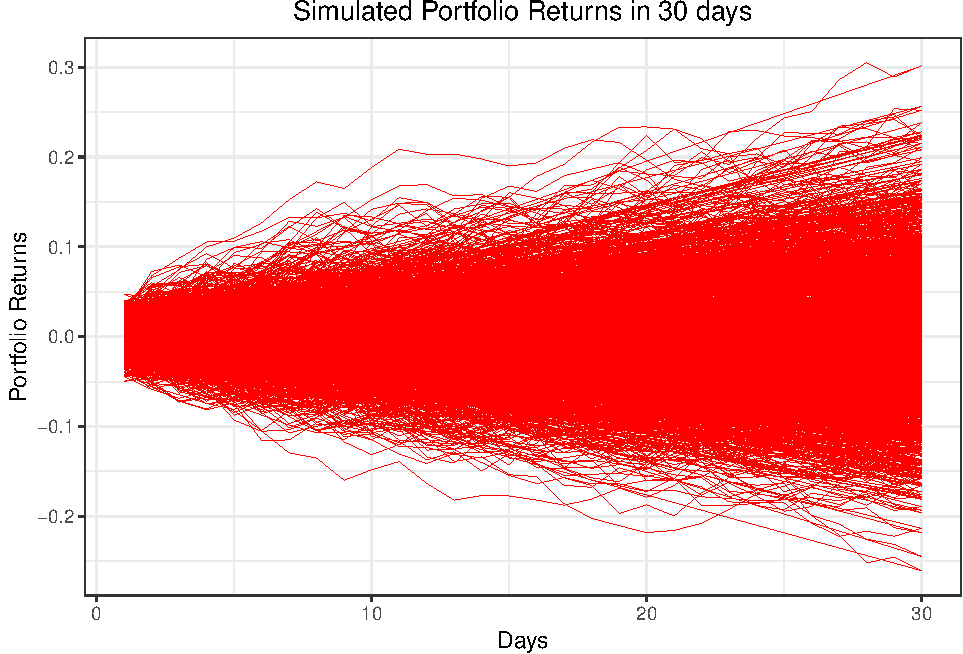
\includegraphics{bookdown_files/figure-latex/R_version_c7-1.pdf}

Get some useful statistics through the results we get

\begin{Shaded}
\begin{Highlighting}[]
\CommentTok{# Porfolio Returns statistics on the 30th day.}
\NormalTok{Avg_Portfolio_Returns =}\StringTok{ }\KeywordTok{mean}\NormalTok{(portfolio_Returns_}\DecValTok{30}\NormalTok{_m[}\DecValTok{30}\NormalTok{,]}\OperatorTok{-}\DecValTok{1}\NormalTok{)}
\NormalTok{SD_Portfolio_Returns =}\StringTok{ }\KeywordTok{sd}\NormalTok{(portfolio_Returns_}\DecValTok{30}\NormalTok{_m[}\DecValTok{30}\NormalTok{,]}\OperatorTok{-}\DecValTok{1}\NormalTok{)}
\NormalTok{Median_Portfolio_Returns =}\StringTok{ }\KeywordTok{median}\NormalTok{(portfolio_Returns_}\DecValTok{30}\NormalTok{_m[}\DecValTok{30}\NormalTok{,]}\OperatorTok{-}\DecValTok{1}\NormalTok{)}
\KeywordTok{print}\NormalTok{(}\KeywordTok{c}\NormalTok{(Avg_Portfolio_Returns,SD_Portfolio_Returns,Median_Portfolio_Returns))}
\end{Highlighting}
\end{Shaded}

\begin{verbatim}
## [1]  0.0009402469  0.0840585273 -0.0015423606
\end{verbatim}

\begin{Shaded}
\begin{Highlighting}[]
\CommentTok{# Construct a 95% Confidential Interval for average returns}
\NormalTok{Avg_CI =}\StringTok{ }\KeywordTok{quantile}\NormalTok{(portfolio_Returns_}\DecValTok{30}\NormalTok{_m[}\DecValTok{30}\NormalTok{,]}\OperatorTok{-}\DecValTok{1}\NormalTok{, }\KeywordTok{c}\NormalTok{(}\FloatTok{0.025}\NormalTok{, }\FloatTok{0.975}\NormalTok{))}
\KeywordTok{print}\NormalTok{(Avg_CI)}
\end{Highlighting}
\end{Shaded}

\begin{verbatim}
##       2.5%      97.5% 
## -0.1541318  0.1702711
\end{verbatim}

\hypertarget{matlab}{%
\subsection{Matlab}\label{matlab}}

Load data and extract stock price

\begin{Shaded}
\begin{Highlighting}[]
\NormalTok{stockData =}\StringTok{ }\KeywordTok{readtable}\NormalTok{(}\StringTok{'./Stats506/Group21_ProjectData.csv'}\NormalTok{);}
\NormalTok{stockPrices =}\StringTok{ }\KeywordTok{table2array}\NormalTok{(}\KeywordTok{stockData}\NormalTok{(}\OperatorTok{:}\NormalTok{, }\DecValTok{2}\OperatorTok{:}\NormalTok{end));}
\end{Highlighting}
\end{Shaded}

Set Monte\_Carlo parameters

\begin{Shaded}
\begin{Highlighting}[]
\NormalTok{mc_rep =}\StringTok{ }\DecValTok{1000}\NormalTok{;}
\NormalTok{initInvestment =}\StringTok{ }\DecValTok{100000}\NormalTok{;}
\NormalTok{numTradingDays =}\StringTok{ }\DecValTok{30}
\end{Highlighting}
\end{Shaded}

Calculate stock returns

\begin{Shaded}
\begin{Highlighting}[]
\NormalTok{stock_returns =}\StringTok{ }\KeywordTok{stock_price}\NormalTok{(}\DecValTok{2}\OperatorTok{:}\NormalTok{end, }\OperatorTok{:}\NormalTok{) .}\OperatorTok{/}\StringTok{ }\KeywordTok{stock_price}\NormalTok{(}\DecValTok{1}\OperatorTok{:}\NormalTok{end}\DecValTok{-1}\NormalTok{, }\OperatorTok{:}\NormalTok{) }\OperatorTok{-}\StringTok{ }\DecValTok{1}\NormalTok{;}
\end{Highlighting}
\end{Shaded}

Set portfolio weight

\begin{Shaded}
\begin{Highlighting}[]
\NormalTok{portfolioWeights =}\StringTok{ }\NormalTok{(}\DecValTok{1}\OperatorTok{/}\DecValTok{3}\NormalTok{) }\OperatorTok{*}\StringTok{ }\KeywordTok{ones}\NormalTok{(}\DecValTok{1}\NormalTok{, }\KeywordTok{size}\NormalTok{(stockPrices,}\DecValTok{2}\NormalTok{));}
\end{Highlighting}
\end{Shaded}

Calculate covariance matrix and mean of the stock returns

\begin{Shaded}
\begin{Highlighting}[]
\NormalTok{% Get the Variance Covariance Matrix of our Stock Returns}
\NormalTok{coVarMat =}\StringTok{ }\KeywordTok{cov}\NormalTok{(stockReturns);}

\NormalTok{% Average returns of each asset }
\NormalTok{mu =}\StringTok{ }\KeywordTok{transpose}\NormalTok{(}\KeywordTok{mean}\NormalTok{(stockReturns));}
\NormalTok{mu =}\StringTok{ }\KeywordTok{repmat}\NormalTok{(mu, }\DecValTok{1}\NormalTok{, numTradingDays);}
\end{Highlighting}
\end{Shaded}

Then we use Monte-Carlo to simulate the portfolio returns in 30 days

\begin{Shaded}
\begin{Highlighting}[]
\ControlFlowTok{for}\NormalTok{ i =}\StringTok{ }\DecValTok{1}\OperatorTok{:}\NormalTok{mc_rep}
\NormalTok{    % }\StringTok{'Randomly generated numbers from N(0,1) distribution'}
\NormalTok{    Z =}\StringTok{ }\KeywordTok{randn}\NormalTok{(}\KeywordTok{size}\NormalTok{(stockReturns,}\DecValTok{2}\NormalTok{), numTradingDays);}

\NormalTok{    % }\StringTok{'Lower Triangular Matrix from Choleski Factorization'}
\NormalTok{    L =}\StringTok{ }\KeywordTok{chol}\NormalTok{(coVarMat, }\StringTok{'lower'}\NormalTok{);}

\NormalTok{    % }\StringTok{'Calculate daily returns for 30 days'}
\NormalTok{    dailyReturns =}\StringTok{ }\NormalTok{mu }\OperatorTok{+}\StringTok{ }\NormalTok{(L }\OperatorTok{*}\StringTok{ }\NormalTok{Z);}

\NormalTok{    % }\StringTok{'Portfolio Returns'}
\NormalTok{    thirtyDayReturn =}\StringTok{ }\KeywordTok{transpose}\NormalTok{(}\KeywordTok{cumprod}\NormalTok{(portfolioWeights }\OperatorTok{*}\StringTok{ }\NormalTok{dailyReturns }\OperatorTok{+}\StringTok{ }\DecValTok{1}\NormalTok{));}
    
\NormalTok{    % }\StringTok{'Add return to the set of all 30-day portfolio returns'}
    \KeywordTok{portfolio30DayReturn_m}\NormalTok{(}\OperatorTok{:}\NormalTok{,i) =}\StringTok{ }\NormalTok{thirtyDayReturn;}
\NormalTok{end}
\end{Highlighting}
\end{Shaded}

Visualizing the result

\begin{Shaded}
\begin{Highlighting}[]
\KeywordTok{plot}\NormalTok{(portfolio30DayReturn_m }\OperatorTok{-}\StringTok{ }\DecValTok{1}\NormalTok{, }\StringTok{'LineWidth'}\NormalTok{, }\FloatTok{0.5}\NormalTok{, }\StringTok{'Color'}\NormalTok{, [}\DecValTok{0}\NormalTok{,}\FloatTok{0.7}\NormalTok{,}\FloatTok{0.9}\NormalTok{, }\FloatTok{0.2}\NormalTok{])}
\KeywordTok{title}\NormalTok{(}\StringTok{'Simulated Portfolio Returns in 30 days'}\NormalTok{, }\StringTok{'fontsize'}\NormalTok{, }\DecValTok{16}\NormalTok{)}
\KeywordTok{xlabel}\NormalTok{(}\StringTok{'Days'}\NormalTok{,}\StringTok{'fontsize'}\NormalTok{,}\DecValTok{16}\NormalTok{)}
\KeywordTok{ylabel}\NormalTok{(}\StringTok{'Portfolio Returns'}\NormalTok{,}\StringTok{'fontsize'}\NormalTok{,}\DecValTok{16}\NormalTok{)}
\end{Highlighting}
\end{Shaded}

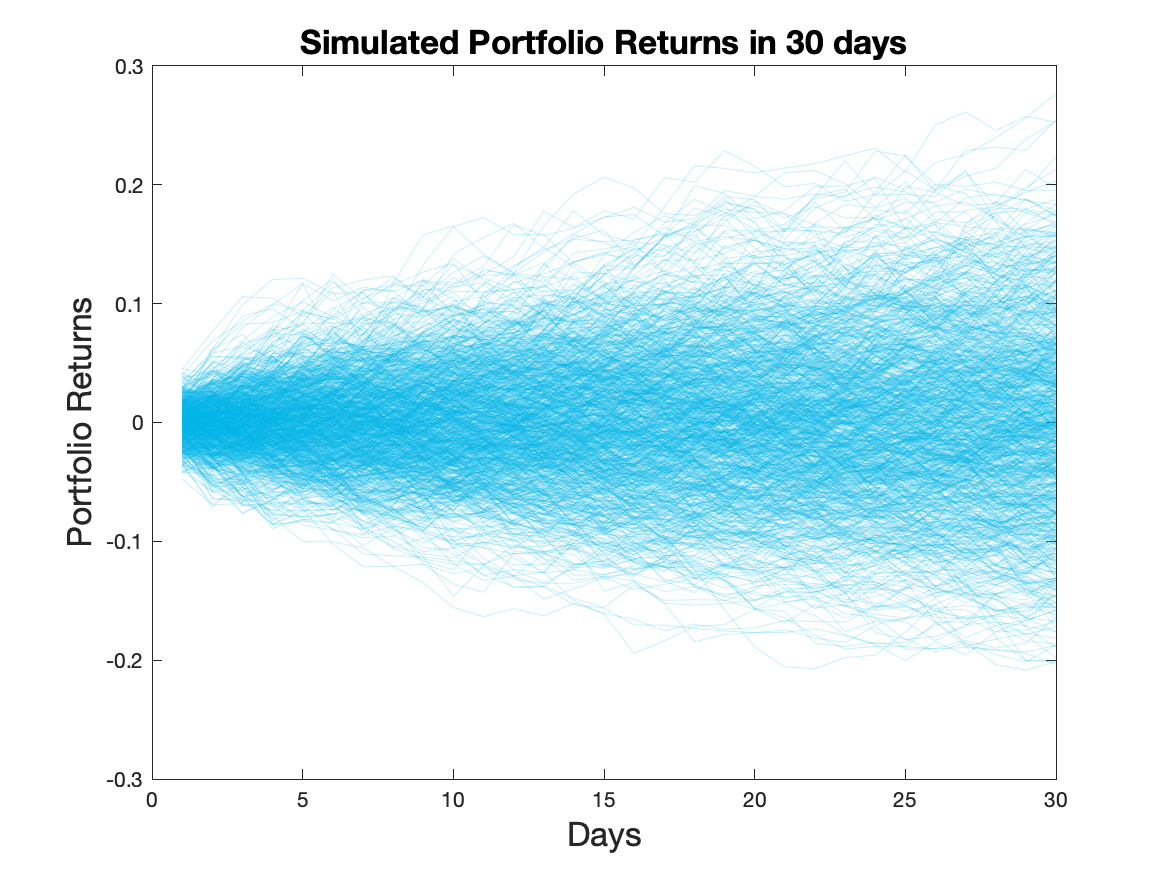
\includegraphics{./Stats506/matlab_pics/ThirtyDay_Returns_Matlab_MC.png}
Finally, we want to get some useful statistics:

\begin{Shaded}
\begin{Highlighting}[]
\NormalTok{% Calculate some statistics }\ControlFlowTok{for}\NormalTok{ our simulated portfolio returns}
\NormalTok{averagePortfolioReturns =}\StringTok{ }\KeywordTok{mean}\NormalTok{(}\KeywordTok{portfolio30DayReturn_m}\NormalTok{(end,}\OperatorTok{:}\NormalTok{) }\OperatorTok{-}\StringTok{ }\DecValTok{1}\NormalTok{);}
\NormalTok{stdDevPortfolioReturns =}\StringTok{ }\KeywordTok{std}\NormalTok{(}\KeywordTok{portfolio30DayReturn_m}\NormalTok{(end,}\OperatorTok{:}\NormalTok{) }\OperatorTok{-}\StringTok{ }\DecValTok{1}\NormalTok{);}
\NormalTok{medianPortfolioReturns =}\StringTok{ }\KeywordTok{median}\NormalTok{(}\KeywordTok{portfolio30DayReturn_m}\NormalTok{(end,}\OperatorTok{:}\NormalTok{) }\OperatorTok{-}\StringTok{ }\DecValTok{1}\NormalTok{);}

\OperatorTok\StringTok{ }\NormalTok{Confidential Interval }\ControlFlowTok{for}\NormalTok{ average returns}

\NormalTok{average_CI =}\StringTok{ }\KeywordTok{quantile}\NormalTok{(}\KeywordTok{portfolio30DayReturn_m}\NormalTok{(end,}\OperatorTok{:}\NormalTok{) }\OperatorTok{-}\StringTok{ }\DecValTok{1}\NormalTok{, [}\FloatTok{0.025}\NormalTok{, }\FloatTok{0.975}\NormalTok{]);}
\end{Highlighting}
\end{Shaded}

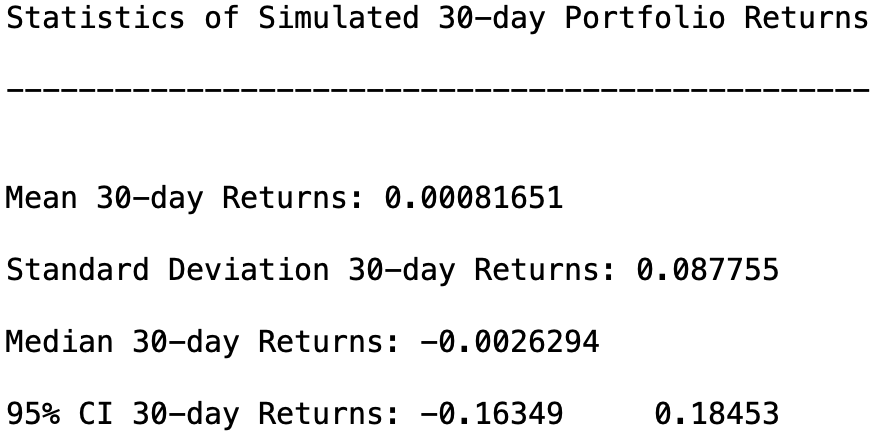
\includegraphics[width=400px]{./Stats506/matlab_pics/Matlab_Simulation_Stats}

\hypertarget{python}{%
\subsection{Python}\label{python}}

Load modules

\begin{Shaded}
\begin{Highlighting}[]
\NormalTok{import pandas as pd}
\NormalTok{import numpy as np}
\NormalTok{import matplotlib.pyplot as plt}
\end{Highlighting}
\end{Shaded}

Load data and extract stock price

\begin{Shaded}
\begin{Highlighting}[]
\NormalTok{stock_data =}\StringTok{ }\KeywordTok{pd.read_csv}\NormalTok{(}\StringTok{"./Stats506/Group21_ProjectData.csv"}\NormalTok{)}
\NormalTok{stock_price =}\StringTok{ }\NormalTok{stock_data.iloc[}\OperatorTok{:}\NormalTok{,}\DecValTok{1}\OperatorTok{:}\DecValTok{4}\NormalTok{]}
\NormalTok{stock_price =}\StringTok{ }\NormalTok{stock_price.values}
\end{Highlighting}
\end{Shaded}

Set Monte\_Carlo parameters

\begin{Shaded}
\begin{Highlighting}[]
\NormalTok{mc_rep =}\StringTok{ }\DecValTok{1000}
\NormalTok{train_days =}\StringTok{ }\DecValTok{30}
\end{Highlighting}
\end{Shaded}

Calculate stock returns

\begin{Shaded}
\begin{Highlighting}[]
\NormalTok{nrows =}\StringTok{ }\KeywordTok{len}\NormalTok{(stock_price)}
\NormalTok{stock_returns =}\StringTok{ }\NormalTok{stock_price[}\DecValTok{1}\OperatorTok{:}\NormalTok{nrows,}\OperatorTok{:}\NormalTok{] }\OperatorTok{/}\StringTok{ }\NormalTok{stock_price[}\DecValTok{0}\OperatorTok{:}\NormalTok{nrows}\DecValTok{-1}\NormalTok{,}\OperatorTok{:}\NormalTok{] }\OperatorTok{-}\StringTok{ }\DecValTok{1}
\end{Highlighting}
\end{Shaded}

Set portfolio weight

\begin{Shaded}
\begin{Highlighting}[]
\NormalTok{portf_WT =}\StringTok{ }\KeywordTok{np.array}\NormalTok{([}\DecValTok{1}\OperatorTok{/}\DecValTok{3}\NormalTok{, }\DecValTok{1}\OperatorTok{/}\DecValTok{3}\NormalTok{, }\DecValTok{1}\OperatorTok{/}\DecValTok{3}\NormalTok{])}
\end{Highlighting}
\end{Shaded}

Calculate covariance matrix and mean of the stock returns

\begin{Shaded}
\begin{Highlighting}[]
\NormalTok{cov =}\StringTok{ }\KeywordTok{np.cov}\NormalTok{(}\KeywordTok{np.transpose}\NormalTok{(stock_returns))}
\NormalTok{miu =}\StringTok{ }\KeywordTok{np.mean}\NormalTok{(stock_returns, }\DataTypeTok{axis=}\DecValTok{0}\NormalTok{)}
\NormalTok{Miu =}\StringTok{ }\KeywordTok{np.full}\NormalTok{((train_days,}\DecValTok{3}\NormalTok{),miu)}
\NormalTok{Miu =}\StringTok{ }\KeywordTok{np.transpose}\NormalTok{(Miu)}
\end{Highlighting}
\end{Shaded}

Then we use Monte-Carlo to simulate the portfolio returns in 30 days

\begin{Shaded}
\begin{Highlighting}[]
\CommentTok{# initial matrix}
\NormalTok{portf_returns_}\DecValTok{30}\NormalTok{_m =}\StringTok{ }\KeywordTok{np.full}\NormalTok{((train_days,mc_rep),}\FloatTok{0.}\NormalTok{)}

\KeywordTok{np.random.seed}\NormalTok{(}\DecValTok{100}\NormalTok{)}
\ControlFlowTok{for}\NormalTok{ i }\ControlFlowTok{in} \KeywordTok{range}\NormalTok{(}\DecValTok{0}\NormalTok{,mc_rep)}\OperatorTok{:}
\StringTok{    }\NormalTok{Z =}\StringTok{ }\KeywordTok{np.random.normal}\NormalTok{(}\DataTypeTok{size=}\DecValTok{3}\OperatorTok{*}\NormalTok{train_days)}
\NormalTok{    Z =}\StringTok{ }\KeywordTok{Z.reshape}\NormalTok{((}\DecValTok{3}\NormalTok{,train_days))}
\NormalTok{    L =}\StringTok{ }\KeywordTok{np.linalg.cholesky}\NormalTok{(cov)}
\NormalTok{    daily_returns =}\StringTok{ }\NormalTok{Miu }\OperatorTok{+}\StringTok{ }\KeywordTok{np.inner}\NormalTok{(L,}\KeywordTok{np.transpose}\NormalTok{(Z))}
\NormalTok{    portf_Returns_}\DecValTok{30}\NormalTok{ =}\StringTok{ }\KeywordTok{np.cumprod}\NormalTok{(}\KeywordTok{np.inner}\NormalTok{(portf_WT,}\KeywordTok{np.transpose}\NormalTok{(daily_returns)) }\OperatorTok{+}\StringTok{ }\DecValTok{1}\NormalTok{)}
\NormalTok{    portf_returns_}\DecValTok{30}\NormalTok{_m[}\OperatorTok{:}\NormalTok{,i] =}\StringTok{ }\NormalTok{portf_Returns_}\DecValTok{30}
\end{Highlighting}
\end{Shaded}

Visualizing the result

\begin{Shaded}
\begin{Highlighting}[]
\KeywordTok{plt.plot}\NormalTok{(portf_returns_}\DecValTok{30}\NormalTok{_m)}
\KeywordTok{plt.ylabel}\NormalTok{(}\StringTok{'Portfolio Returns'}\NormalTok{)}
\KeywordTok{plt.xlabel}\NormalTok{(}\StringTok{'Days'}\NormalTok{)}
\KeywordTok{plt.title}\NormalTok{(}\StringTok{'Simulated Portfolio Returns in 30 days'}\NormalTok{)}
\KeywordTok{plt.show}\NormalTok{()}
\end{Highlighting}
\end{Shaded}

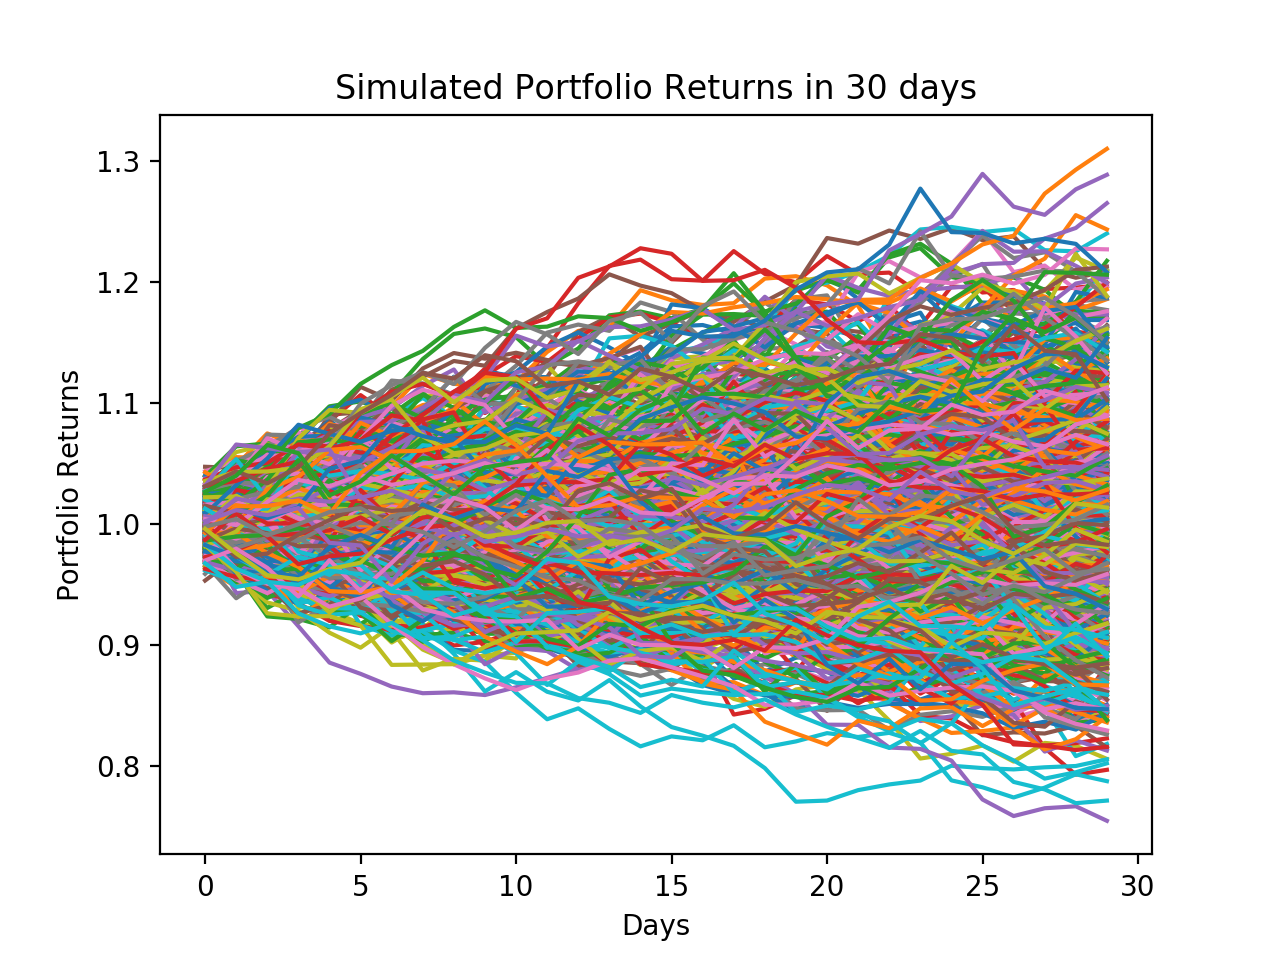
\includegraphics{./Stats506/Python_pics/Portf_returns_py.png}
Finally, we want to get some useful statistics:

\begin{Shaded}
\begin{Highlighting}[]
\CommentTok{# Porfolio Returns statistics on the 30th day}
\NormalTok{Avg_portf_returns =}\StringTok{ }\KeywordTok{np.mean}\NormalTok{(portf_returns_}\DecValTok{30}\NormalTok{_m[}\DecValTok{29}\NormalTok{,}\OperatorTok{:}\NormalTok{]}\OperatorTok{-}\DecValTok{1}\NormalTok{)}
\NormalTok{SD_portf_returns =}\StringTok{ }\KeywordTok{np.std}\NormalTok{(portf_returns_}\DecValTok{30}\NormalTok{_m[}\DecValTok{29}\NormalTok{,}\OperatorTok{:}\NormalTok{]}\OperatorTok{-}\DecValTok{1}\NormalTok{)}
\NormalTok{Median_portf_returns =}\StringTok{ }\KeywordTok{np.median}\NormalTok{(portf_returns_}\DecValTok{30}\NormalTok{_m[}\DecValTok{29}\NormalTok{,}\OperatorTok{:}\NormalTok{]}\OperatorTok{-}\DecValTok{1}\NormalTok{)}
\KeywordTok{print}\NormalTok{(Avg_portf_returns)}
\KeywordTok{print}\NormalTok{(SD_portf_returns)}
\KeywordTok{print}\NormalTok{(Median_portf_returns)}
\end{Highlighting}
\end{Shaded}

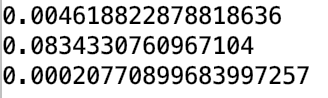
\includegraphics[width=200px]{./Stats506/Python_pics/avgsdmedian}

\begin{Shaded}
\begin{Highlighting}[]
\CommentTok{# construct CI for average}
\NormalTok{Avg_CI =}\StringTok{ }\KeywordTok{np.quantile}\NormalTok{(portf_returns_}\DecValTok{30}\NormalTok{_m[}\DecValTok{29}\NormalTok{,}\OperatorTok{:}\NormalTok{]}\OperatorTok{-}\DecValTok{1}\NormalTok{,}\KeywordTok{np.array}\NormalTok{([}\FloatTok{0.025}\NormalTok{,}\FloatTok{0.975}\NormalTok{]))}
\KeywordTok{print}\NormalTok{(Avg_CI)}
\end{Highlighting}
\end{Shaded}

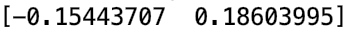
\includegraphics[width=200px]{./Stats506/Python_pics/CI}

\hypertarget{results}{%
\section{Results}\label{results}}

For our particular example, the portfolio returns averaged over all monte carlo
trials had an average close to 0. The reason the average is close to 0 is
because Apple, Facebook, and Google have average returns close to 0 over the past year.
Therefore, our simulated returns essentially had no drift. Also, assuming a
normal distribution of the returns would not work well in practice since
stock returns are typically fat-tailed and not normally distributed. However, based on our
Monte Carlo Study, we do not suggest investing in this portfolio based on the
low expected portfolio returns.

\hypertarget{note}{%
\section{Note}\label{note}}

Statistics we get using three different languages are slightly different, because in our simulation
process, we have generated random numbers and these numbers cannot be exactly identical.

\hypertarget{reference}{%
\section{Reference}\label{reference}}

\emph{Yahoo Finance}

\hypertarget{my-readme}{%
\chapter{My Readme}\label{my-readme}}

This is a minimal example of a book based on R Markdown and \textbf{bookdown} (\url{https://github.com/rstudio/bookdown}). Please see the page ``Get Started'' at \url{https://bookdown.org/} for how to compile this example.

\hypertarget{literature}{%
\chapter{Literature}\label{literature}}

Here is a review of existing methods.

\bibliography{book.bib,packages.bib}


\end{document}
